\begin{figure}
\centerline{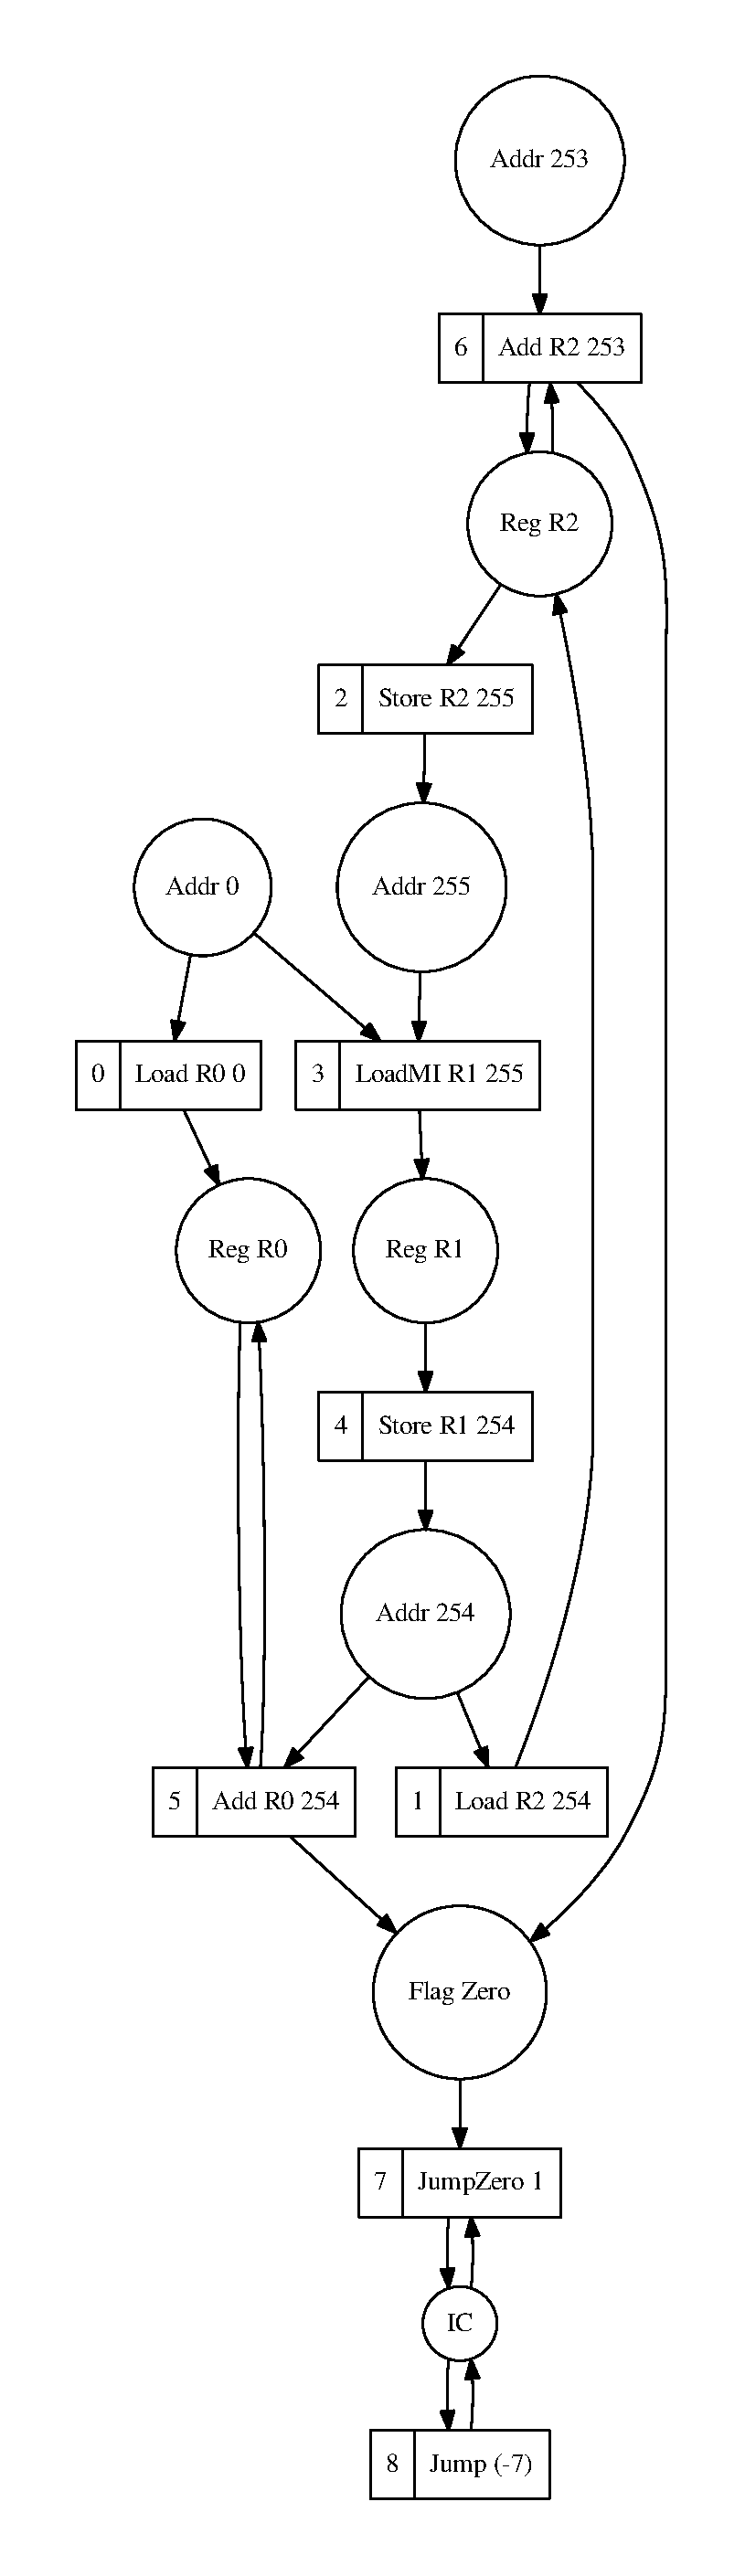
\includegraphics[scale=0.45]{img/sumArray.pdf}}
\caption{Approximation of static dependencies of an array summation program.\label{fig-sum}}
\end{figure}

The paper presented a polymorphic metalanguage for describing the semantics of
a generic instruction set architecture.
% The metalanguage closely resembles state
% transformers.
The polymorphism of the metalanguage terms allows us to evaluate the semantics
of instructions in different contexts without any modification of the semantics
itself. As the primary application, we present an approach to deriving
concurrency oracles of the instructions with only static data dependencies.

To handle instructions whose dependencies are dynamic, it is possible to use
conservative approximation of dependencies. For example, Fig.~\ref{fig-sum}
shows a dependency graph for a small array summation program that contains
a conditional branch instruction \hs{JumpZero} which modifies the instruction
counter \hs{IC} only if the previous instruction set the \hs{Zero} flag. In
this example we conservatively assume that \hs{JumpZero} always has a dependency
on \hs{IC}.

